\section{Combinazione agli SLU}
Il \textbf{capitolo 2.5.3} delle \emph{NTC 2018} descrive, ai fini delle verifiche agli stati limite, le varie combinazioni delle azioni. 

La combinazione fondamentale, impiegata per il calcolo agli \emph{stati limite ultimi} è descritta dalla \emph{[2.5.1]} ed è così formulata
\[
	\gamma_{G1}\cdot G_{1k} + \gamma_{G2}\cdot G_{2k} + \gamma_{Q1} \cdot Q_{1k} + \gamma_{Q2}\cdot \psi_{02}\cdot Q_{2k} + \gamma_{Q3}\cdot \psi_{03}\cdot Q_{3k} + \dots
\]

Si riportano di seguito il calcolo dei carichi distribuiti secondo la formulazione agli SLU, in funzione dei tratti di trave in esame.

Ricordando che si sta trattando una trave di bordo, saranno necessarie diverse combinazioni di carico per valutare la massima azione sulla trave. È comunque evidente che sovraccarichi di minor rilevanza, in termini di azione, daranno un contributo molto minore rispetto a sovraccarichi più elevati. Verranno tralasciati, pertanto, le combinazioni ove questi sovraccarichi risultano essere principali.

\subsection{Calcolo delle azioni massime e minime}

\subsubsection*{Tratto $P13\div P16$}
Dalla tabella~\ref{tab:azioniTrave} si può vedere che i carichi che generano un'azione di maggior rilievo sono quelli di categoria (B) della terrazza e il carico da neve. Verranno, perciò, calcolate due sole combinazioni.

\paragraph{Combinazione 1: neve principale}
Nella combinazione per cui l'azione della neve è principale, le altre azioni saranno ridotte di un fattore che dipende dalla categoria di cui fanno parte.

\begin{align*}
	Q_{11}^{max} &=\gamma_{G1_{SF}}\cdot\left( G_{1k, interno} + G_{1k, terrazza} + G_{1k, trave} \right) +\\
	&+\gamma_{G2_{SF}}\cdot\left( G_{2k, interno} + G_{2k, terrazza} + G_{2k, tamponamento} \right) +\\
	&+\gamma_{Q_{SF}}\cdot (Q_{neve} + \psi_{0,CAT.B2,int}\cdot Q_{CAT.B2,int} + \psi_{0,CAT.B2,terr}\cdot Q_{CAT.B2,terr} +\\
	&+\psi_{0,vento}\cdot Q_{vento}) =\\
	&= 1.3\cdot(8+11.52 + 3.75)	+1.5\cdot(11.55+7.98 + 9.20) + 1.5\cdot(15.01) +\\
	&+1.5\cdot(0.7\cdot7.5+ 0.7\cdot 14.40 + 0.6\cdot 0.5) = \\
	&= 	119.306\,\dfrac{kN}{m}
\end{align*}






\paragraph{Combinazione 2: categoria B2 (terrazza) principale}

\begin{align*}
	Q_{12}^{max} &= 1.3\cdot(8+11.52 + 3.75) 
	+1.5\cdot(11.55+7.98 + 9.20) +\\
	&+1.5\cdot(0.5\cdot 15.01 + 0.7\cdot7.5+ 14.40 + 0.6\cdot 0.5) = \\
	&= 	114.345\,\dfrac{kN}{m}
\end{align*}

\paragraph{Combinazione 3: vento principale}
Per valutare il minimo, viene considerata l'azione del vento che 'alleggerisce' la trave, quella cioè con valore negativo.

\begin{align*}
	Q_{13}^{min} &=\gamma_{G1_{F}}\cdot\left( G_{1k, interno} + G_{1k, terrazza} + G_{1k, trave} \right) +\\
	&+\gamma_{G2_{F}}\cdot\left( G_{2k, interno} + G_{2k, terrazza} + G_{2k, tamponamento} \right) +\\
	&+\gamma_{Q_{F}}\cdot (\psi_{0,neve}\cdot Q_{neve} + \psi_{0,CAT.B2,int}\cdot Q_{CAT.B2,int} + \psi_{0,CAT.B2,terr}\cdot Q_{CAT.B2,terr}) +\\
	&+ \gamma_{vento_{SF}}\cdot Q_{vento} =\\
	&= 1\cdot(8+11.52 + 3.75) +0.8 \cdot(11.55+7.98 + 9.20) +\\
	&+ 0\cdot(0.5\cdot 15.01 + 0.7\cdot7.5+ 0.7\cdot 10.80) - 1.5\cdot 0.5 = \\
	&= 	45.50\,\dfrac{kN}{m}
\end{align*}

I valori massimo e minimo sul primo tratto di trave per la combinazione agli SLU sono rispettivamente la combinazione con il carico da neve principale e la combinazione con l'azione del vento principale.

\begin{equation}
		\label{eq:Q1maxmin_slu}
		\begin{cases}
			Q_{1,max} = 119.306\,\dfrac{kN}{m}\\\\
			Q_{1, min} = 45.50\,\dfrac{kN}{m}
		\end{cases}
\end{equation}

\subsubsection*{Tratto $P16\div P17$}

\paragraph{Combinazione 1: neve principale}

\begin{align*}
	Q_{21}^{max} &= 1.3\cdot(8.00 +6.72 + 3.75) + 1.5\cdot(11.55+4.65 + 9.20) + 1.5\cdot(10.30)+\\
	&+ 1.5\cdot0.7\cdot(7.50+8.40) + 1.5\cdot0.6\cdot0.3 =\\
	&= 	94.526\,\dfrac{kN}{m}
\end{align*}

\paragraph{Combinazione 2: categoria B2 (terrazza) principale}

\begin{align*}
	Q_{22}^{max} &= 1.3\cdot(8.00 +6.72 + 3.75) + 1.5\cdot(11.55+4.65 + 9.20) + 1.5\cdot8.40+\\
	&+ 1.5\cdot(0.7\cdot7.50+ 0.5\cdot 10.30 + 0.6\cdot0.3) =\\
	&= 	90.581\,\dfrac{kN}{m}
\end{align*}

\paragraph{Combinazione 3: vento principale}

\begin{align*}
	Q_{23}^{min} &= 1\cdot(8.00 +6.72 + 3.75) + 0.8\cdot(11.55+4.65 + 9.20) +\\
	&+ 0\cdot(0.7\cdot 8.40 + 0.7\cdot7.50+ 0.5\cdot 10.30) -1.5\cdot0.3 =\\
	&= 	38.34\,\dfrac{kN}{m}
\end{align*}

Come nel tratto precedente, il massimo e il minimo coincidono con la combinazione con neve principale e la combinazione con vento principale.

\begin{equation}
		\label{eq:Q2maxmin_slu}
		\begin{cases}
			Q_{2,max} = 94.526\,\dfrac{kN}{m}\\\\
			Q_{2, min} = 38.34\,\dfrac{kN}{m}
		\end{cases}
\end{equation}

\subsubsection*{Tratto $P17$ - vano scala}

\paragraph{Combinazione 1: neve principale}

\begin{align*}
	Q_{31}^{max} &= 1.3\cdot(6.00+3.20 + 3.75) + 1.5\cdot(8.66+2.215 + 9.20) + 1.5\cdot(4.17) +\\
	&+1.5\cdot0.7\cdot(5.63+4.00) + 1.5\cdot0.6\cdot0.138 =\\
	&= 	63.44\,\dfrac{kN}{m}
\end{align*}

\paragraph{Combinazione 2: categoria B2 (terrazza) principale}

\begin{align*}
	Q_{32}^{max} &= 1.3\cdot(6.00+3.20 + 3.75) + 1.5\cdot(8.66+2.215 + 9.20) + 1.5\cdot(4.00) +\\
	&+1.5\cdot(0.7\cdot5.63+ 0.5\cdot4.17 + 0.6\cdot 0.138) =\\
	&=  62.11\,\dfrac{kN}{m}
\end{align*}

\paragraph{Combinazione 3: categoria B2 (interno) principale}

\begin{align*}
	Q_{33}^{max} &= 1.3\cdot(6.00+3.20 + 3.75) + 1.5\cdot(8.66+2.215 + 9.20) + 1.5\cdot(5.63) +\\
	&+1.5\cdot(0.7\cdot4.00+ 0.5\cdot4.17 + 0.6\cdot 0.138) =\\
	&=  62.84\,\dfrac{kN}{m}
\end{align*}

\paragraph{Combinazione 4: vento principale}

\begin{align*}
	Q_{34}^{min} &= 1\cdot(6.00+3.20 + 3.75) + 0.8\cdot(8.66+2.215 + 9.20) +\\
	&+0\cdot(0.7 \cdot 5.63 + 0.7\cdot4.00+ 0.5\cdot4.17) - 1.5\cdot 0.138 =\\
	&=  28.80\,\dfrac{kN}{m}
\end{align*}

I valori massimo e minimo sono

\begin{equation}
		\label{eq:Q3maxmin_slu}
		\begin{cases}
			Q_{3,max} = 63.44\,\dfrac{kN}{m}\\\\
			Q_{3, min} = 28.80\,\dfrac{kN}{m}
		\end{cases}
\end{equation}

\subsection{Combinazioni di carico}\label{sec:loadCombo}
Sostituendo ora i valori trovati nelle \eqref{eq:Q1maxmin_slu}, \eqref{eq:Q2maxmin_slu} e \eqref{eq:Q3maxmin_slu} all'interno della tabella~\ref{tab:loadCombo} di pagina~\pageref{tab:loadCombo} si possono trovare le otto combinazioni di carico che massimizzano le azioni interne.

\begin{figure}
     \centering
     \subfloat[\emph{Combinazione 1: MAX-MIN-MAX-MIN-MAX-MIN}]{
 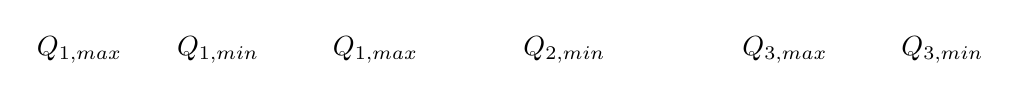
\begin{tikzpicture}[xscale=.8]
 \scaling{.48};
  \point{p13}{0}{0};
  \point{p14}{3}{0};
  \point{p15}{7.5}{0};
  \point{p16}{11.5}{0};
  \point{p17}{16.5}{0};
  \point{p18}{22.65}{0};
  \point{vs}{26.65}{0};
  
  \beam{1}{p13}{vs};
  
  \support{1}{p13};
  \support{2}{p14};
  \support{2}{p15};
  \support{2}{p16};
  \support{2}{p17};
  \support{2}{p18};
  \support{2}{vs};
  
    
   
    \node at (0.8,1.8) {$Q_{1,max}$};
    \node at (3,1.8) {$Q_{1,min}$};
    \node at (5.5,1.8) {$Q_{1,max}$};
    \node at (8.5,1.8) {$Q_{2,min}$};
    \node at (12,1.8) {$Q_{3,max}$};
    \node at (14.5,1.8) {$Q_{3,min}$};
    
    \lineload{1}{p13}{p14}[1.2][1.2][.08];
    \lineload{1}{p14}{p15}[.45][.45][.08];
    \lineload{1}{p15}{p16}[1.2][1.2][.08];
    \lineload{1}{p16}{p17}[.38][.38][.08];
    \lineload{1}{p17}{p18}[.73][.73][.08];
    \lineload{1}{p18}{vs}[.33][.33][.08];

 \end{tikzpicture}\label{fig:sluCombo_1}}\\
 %
 \subfloat[\emph{Combinazione 2: MAX-MAX-MIN-MAX-MIN-MAX}]{
 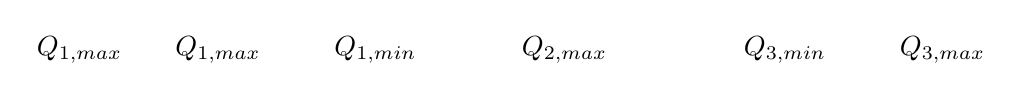
\begin{tikzpicture}[xscale=.8]
 \scaling{.48};
  \point{p13}{0}{0};
  \point{p14}{3}{0};
  \point{p15}{7.5}{0};
  \point{p16}{11.5}{0};
  \point{p17}{16.5}{0};
  \point{p18}{22.65}{0};
  \point{vs}{26.65}{0};
  
  \beam{1}{p13}{vs};
  
  \support{1}{p13};
  \support{2}{p14};
  \support{2}{p15};
  \support{2}{p16};
  \support{2}{p17};
  \support{2}{p18};
  \support{2}{vs};
  
    
   
    \node at (0.8,1.8) {$Q_{1,max}$};
    \node at (3,1.8) {$Q_{1,max}$};
    \node at (5.5,1.8) {$Q_{1,min}$};
    \node at (8.5,1.8) {$Q_{2,max}$};
    \node at (12,1.8) {$Q_{3,min}$};
    \node at (14.5,1.8) {$Q_{3,max}$};
    
    \lineload{1}{p13}{p14}[1.2][1.2][.08];
    \lineload{1}{p14}{p15}[1.2][1.2][.08];
    \lineload{1}{p15}{p16}[.45][.45][.08];
    \lineload{1}{p16}{p17}[.95][.95][.08];
    \lineload{1}{p17}{p18}[.33][.33][.08];
    \lineload{1}{p18}{vs}[.73][.73][.08];

 \end{tikzpicture}\label{fig:sluCombo_2}}\\
 %
 \subfloat[\emph{Combinazione 3: MIN-MAX-MIN-MAX-MIN-MAX}]{
 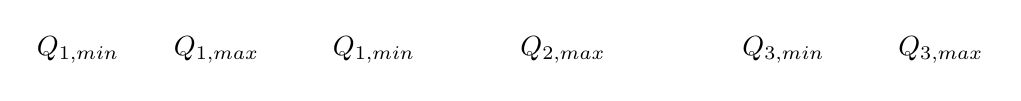
\begin{tikzpicture}[xscale=.8]
 \scaling{.48};
  \point{p13}{0}{0};
  \point{p14}{3}{0};
  \point{p15}{7.5}{0};
  \point{p16}{11.5}{0};
  \point{p17}{16.5}{0};
  \point{p18}{22.65}{0};
  \point{vs}{26.65}{0};
  
  \beam{1}{p13}{vs};
  
  \support{1}{p13};
  \support{2}{p14};
  \support{2}{p15};
  \support{2}{p16};
  \support{2}{p17};
  \support{2}{p18};
  \support{2}{vs};
  
    
   
    \node at (0.8,1.8) {$Q_{1,min}$};
    \node at (3,1.8) {$Q_{1,max}$};
    \node at (5.5,1.8) {$Q_{1,min}$};
    \node at (8.5,1.8) {$Q_{2,max}$};
    \node at (12,1.8) {$Q_{3,min}$};
    \node at (14.5,1.8) {$Q_{3,max}$};
    
    \lineload{1}{p13}{p14}[.45][.45][.08];
    \lineload{1}{p14}{p15}[1.2][1.2][.08];
    \lineload{1}{p15}{p16}[.45][.45][.08];
    \lineload{1}{p16}{p17}[.94][.94][.08];
    \lineload{1}{p17}{p18}[.33][.33][.08];
    \lineload{1}{p18}{vs}[.73][.73][.08];

 \end{tikzpicture}\label{fig:sluCombo_3}}\\
 %
 \subfloat[\emph{Combinazione 4: MIN-MAX-MAX-MIN-MAX-MIN}]{
 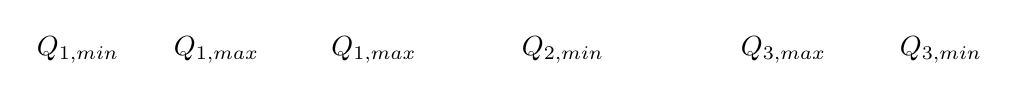
\begin{tikzpicture}[xscale=.8]
 \scaling{.48};
  \point{p13}{0}{0};
  \point{p14}{3}{0};
  \point{p15}{7.5}{0};
  \point{p16}{11.5}{0};
  \point{p17}{16.5}{0};
  \point{p18}{22.65}{0};
  \point{vs}{26.65}{0};
  
  \beam{1}{p13}{vs};
  
  \support{1}{p13};
  \support{2}{p14};
  \support{2}{p15};
  \support{2}{p16};
  \support{2}{p17};
  \support{2}{p18};
  \support{2}{vs};
  
    
   
    \node at (0.8,1.8) {$Q_{1,min}$};
    \node at (3,1.8) {$Q_{1,max}$};
    \node at (5.5,1.8) {$Q_{1,max}$};
    \node at (8.5,1.8) {$Q_{2,min}$};
    \node at (12,1.8) {$Q_{3,max}$};
    \node at (14.5,1.8) {$Q_{3,min}$};
    
    \lineload{1}{p13}{p14}[.45][.45][.08];
    \lineload{1}{p14}{p15}[1.2][1.2][.08];
    \lineload{1}{p15}{p16}[1.2][1.2][.08];
    \lineload{1}{p16}{p17}[.38][.38][.08];
    \lineload{1}{p17}{p18}[.73][.73][.08];
    \lineload{1}{p18}{vs}[.33][.33][.08];

 \end{tikzpicture}\label{fig:sluCombo_4}}
 \caption{Combinazioni di carico (continua nella pagina successiva)}
 \label{fig:loadCombo_1}
\end{figure}

\begin{figure}
\ContinuedFloat
\centering
 %
 \subfloat[\emph{Combinazione 5: MAX-MIN-MAX-MAX-MAX-MIN}]{
 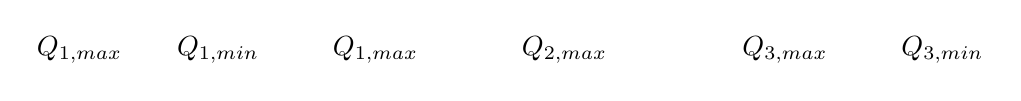
\begin{tikzpicture}[xscale=.8]
 \scaling{.48};
  \point{p13}{0}{0};
  \point{p14}{3}{0};
  \point{p15}{7.5}{0};
  \point{p16}{11.5}{0};
  \point{p17}{16.5}{0};
  \point{p18}{22.65}{0};
  \point{vs}{26.65}{0};
  
  \beam{1}{p13}{vs};
  
  \support{1}{p13};
  \support{2}{p14};
  \support{2}{p15};
  \support{2}{p16};
  \support{2}{p17};
  \support{2}{p18};
  \support{2}{vs};
  
    
   
    \node at (0.8,1.8) {$Q_{1,max}$};
    \node at (3,1.8) {$Q_{1,min}$};
    \node at (5.5,1.8) {$Q_{1,max}$};
    \node at (8.5,1.8) {$Q_{2,max}$};
    \node at (12,1.8) {$Q_{3,max}$};
    \node at (14.5,1.8) {$Q_{3,min}$};
    
    \lineload{1}{p13}{p14}[1.2][1.2][.08];
    \lineload{1}{p14}{p15}[.45][.45][.08];
    \lineload{1}{p15}{p16}[1.2][1.2][.08];
    \lineload{1}{p16}{p17}[.94][.94][.08];
    \lineload{1}{p17}{p18}[.73][.73][.08];
    \lineload{1}{p18}{vs}[.33][.33][.08];

 \end{tikzpicture}\label{fig:sluCombo_5}}\\
 %
 \subfloat[\emph{Combinazione 6: MAX-MIN-MAX-MAX-MIN-MAX}]{
 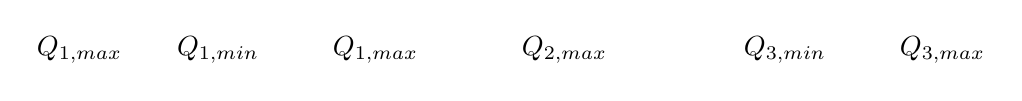
\begin{tikzpicture}[xscale=.8]
 \scaling{.48};
  \point{p13}{0}{0};
  \point{p14}{3}{0};
  \point{p15}{7.5}{0};
  \point{p16}{11.5}{0};
  \point{p17}{16.5}{0};
  \point{p18}{22.65}{0};
  \point{vs}{26.65}{0};
  
  \beam{1}{p13}{vs};
  
  \support{1}{p13};
  \support{2}{p14};
  \support{2}{p15};
  \support{2}{p16};
  \support{2}{p17};
  \support{2}{p18};
  \support{2}{vs};
  
    
   
    \node at (0.8,1.8) {$Q_{1,max}$};
    \node at (3,1.8) {$Q_{1,min}$};
    \node at (5.5,1.8) {$Q_{1,max}$};
    \node at (8.5,1.8) {$Q_{2,max}$};
    \node at (12,1.8) {$Q_{3,min}$};
    \node at (14.5,1.8) {$Q_{3,max}$};
    
    \lineload{1}{p13}{p14}[1.2][1.2][.08];
    \lineload{1}{p14}{p15}[.45][.45][.08];
    \lineload{1}{p15}{p16}[1.2][1.2][.08];
    \lineload{1}{p16}{p17}[.94][.94][.08];
    \lineload{1}{p17}{p18}[.33][.33][.08];
    \lineload{1}{p18}{vs}[.73][.73][.08];

 \end{tikzpicture}\label{fig:sluCombo_6}}\\
 %
 \subfloat[\emph{Combinazione 7: MIN-MAX-MIN-MAX-MAX-MIN}]{
 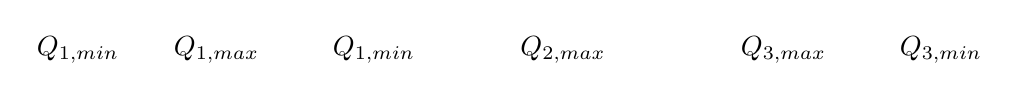
\begin{tikzpicture}[xscale=.8]
 \scaling{.48};
  \point{p13}{0}{0};
  \point{p14}{3}{0};
  \point{p15}{7.5}{0};
  \point{p16}{11.5}{0};
  \point{p17}{16.5}{0};
  \point{p18}{22.65}{0};
  \point{vs}{26.65}{0};
  
  \beam{1}{p13}{vs};
  
  \support{1}{p13};
  \support{2}{p14};
  \support{2}{p15};
  \support{2}{p16};
  \support{2}{p17};
  \support{2}{p18};
  \support{2}{vs};
  
    
   
    \node at (0.8,1.8) {$Q_{1,min}$};
    \node at (3,1.8) {$Q_{1,max}$};
    \node at (5.5,1.8) {$Q_{1,min}$};
    \node at (8.5,1.8) {$Q_{2,max}$};
    \node at (12,1.8) {$Q_{3,max}$};
    \node at (14.5,1.8) {$Q_{3,min}$};
    
    \lineload{1}{p13}{p14}[.45][.45][.08];
    \lineload{1}{p14}{p15}[1.2][1.2][.08];
    \lineload{1}{p15}{p16}[.45][.45][.08];
    \lineload{1}{p16}{p17}[.94][.94][.08];
    \lineload{1}{p17}{p18}[.73][.73][.08];
    \lineload{1}{p18}{vs}[.33][.33][.08];

 \end{tikzpicture}\label{fig:sluCombo_7}}\\
 %
 \subfloat[\emph{Combinazione 8: MAX-MIN-MAX-MIN-MAX-MAX}]{
 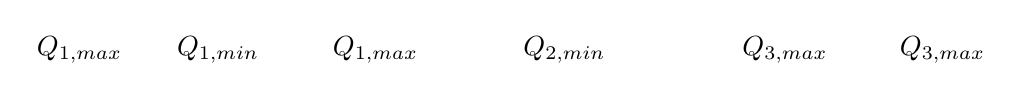
\begin{tikzpicture}[xscale=.8]
 \scaling{.48};
  \point{p13}{0}{0};
  \point{p14}{3}{0};
  \point{p15}{7.5}{0};
  \point{p16}{11.5}{0};
  \point{p17}{16.5}{0};
  \point{p18}{22.65}{0};
  \point{vs}{26.65}{0};
  
  \beam{1}{p13}{vs};
  
  \support{1}{p13};
  \support{2}{p14};
  \support{2}{p15};
  \support{2}{p16};
  \support{2}{p17};
  \support{2}{p18};
  \support{2}{vs};
  
    
   
    \node at (0.8,1.8) {$Q_{1,max}$};
    \node at (3,1.8) {$Q_{1,min}$};
    \node at (5.5,1.8) {$Q_{1,max}$};
    \node at (8.5,1.8) {$Q_{2,min}$};
    \node at (12,1.8) {$Q_{3,max}$};
    \node at (14.5,1.8) {$Q_{3,max}$};
    
    \lineload{1}{p13}{p14}[1.2][1.2][.08];
    \lineload{1}{p14}{p15}[0.45][.45][.08];
    \lineload{1}{p15}{p16}[1.2][1.2][.08];
    \lineload{1}{p16}{p17}[.38][.38][.08];
    \lineload{1}{p17}{p18}[.73][.73][.08];
    \lineload{1}{p18}{vs}[.73][.73][.08];

 \end{tikzpicture}\label{fig:sluCombo_8}}
 \smallskip
 \caption{Combinazioni di carico (continua dalla pagina precedente)}
 \label{fig:loadCombo_2}
 \end{figure}
 
 Le otto combinazioni di carico massimizzano il momento flettente su, in ordine, la prima campata ($C1$), il secondo appoggio ($N2$), la seconda campata ($C2$), il terzo appoggio ($N3$) e così via. Le combinazioni sono state integrate nel codice come segue; ad esempio, per la prima combinazione:
 \cleardoublepage
 \begin{lstlisting}[language=Python]
s = np.linspace(0,26.65, num=1000)
MC1 = M1*Q1max_slu + M2*Q1min_slu + M3*Q1max_slu + M4*Q2min_slu + M5*Q3max_slu + M6*Q3min_slu

#----------PLOT------------------

plt.figure(figsize=(20,10))
plt.plot(s, MC1, color='blue')
plt.xlim(s.min(), s.max())
plt.gca().invert_yaxis()
plt.grid()
plt.xlabel(r'$s\,[m]$', fontsize='14')
plt.ylabel(r'$M_{C1}(s)\,[kN\,m]$', fontsize='14')
plt.xticks([0, 3, 7.5, 11.5, 16.5, 22.65, 26.65])
plt.axhline(0, color='black')
plt.title('Momento Flettente\nCombinazione 1: MAX-MIN-MAX-MIN-MAX-MIN', fontsize='22')
plt.savefig('export/img/bendingMomentCombo_1.jpg')
plt.show()
 \end{lstlisting}
 \noindent
Il codice sopra riportato genera il diagramma del momento flettente rappresentato in figura~\ref{fig:bendingMomentCombo_1}.
 
 \begin{figure}
 	\centering
 	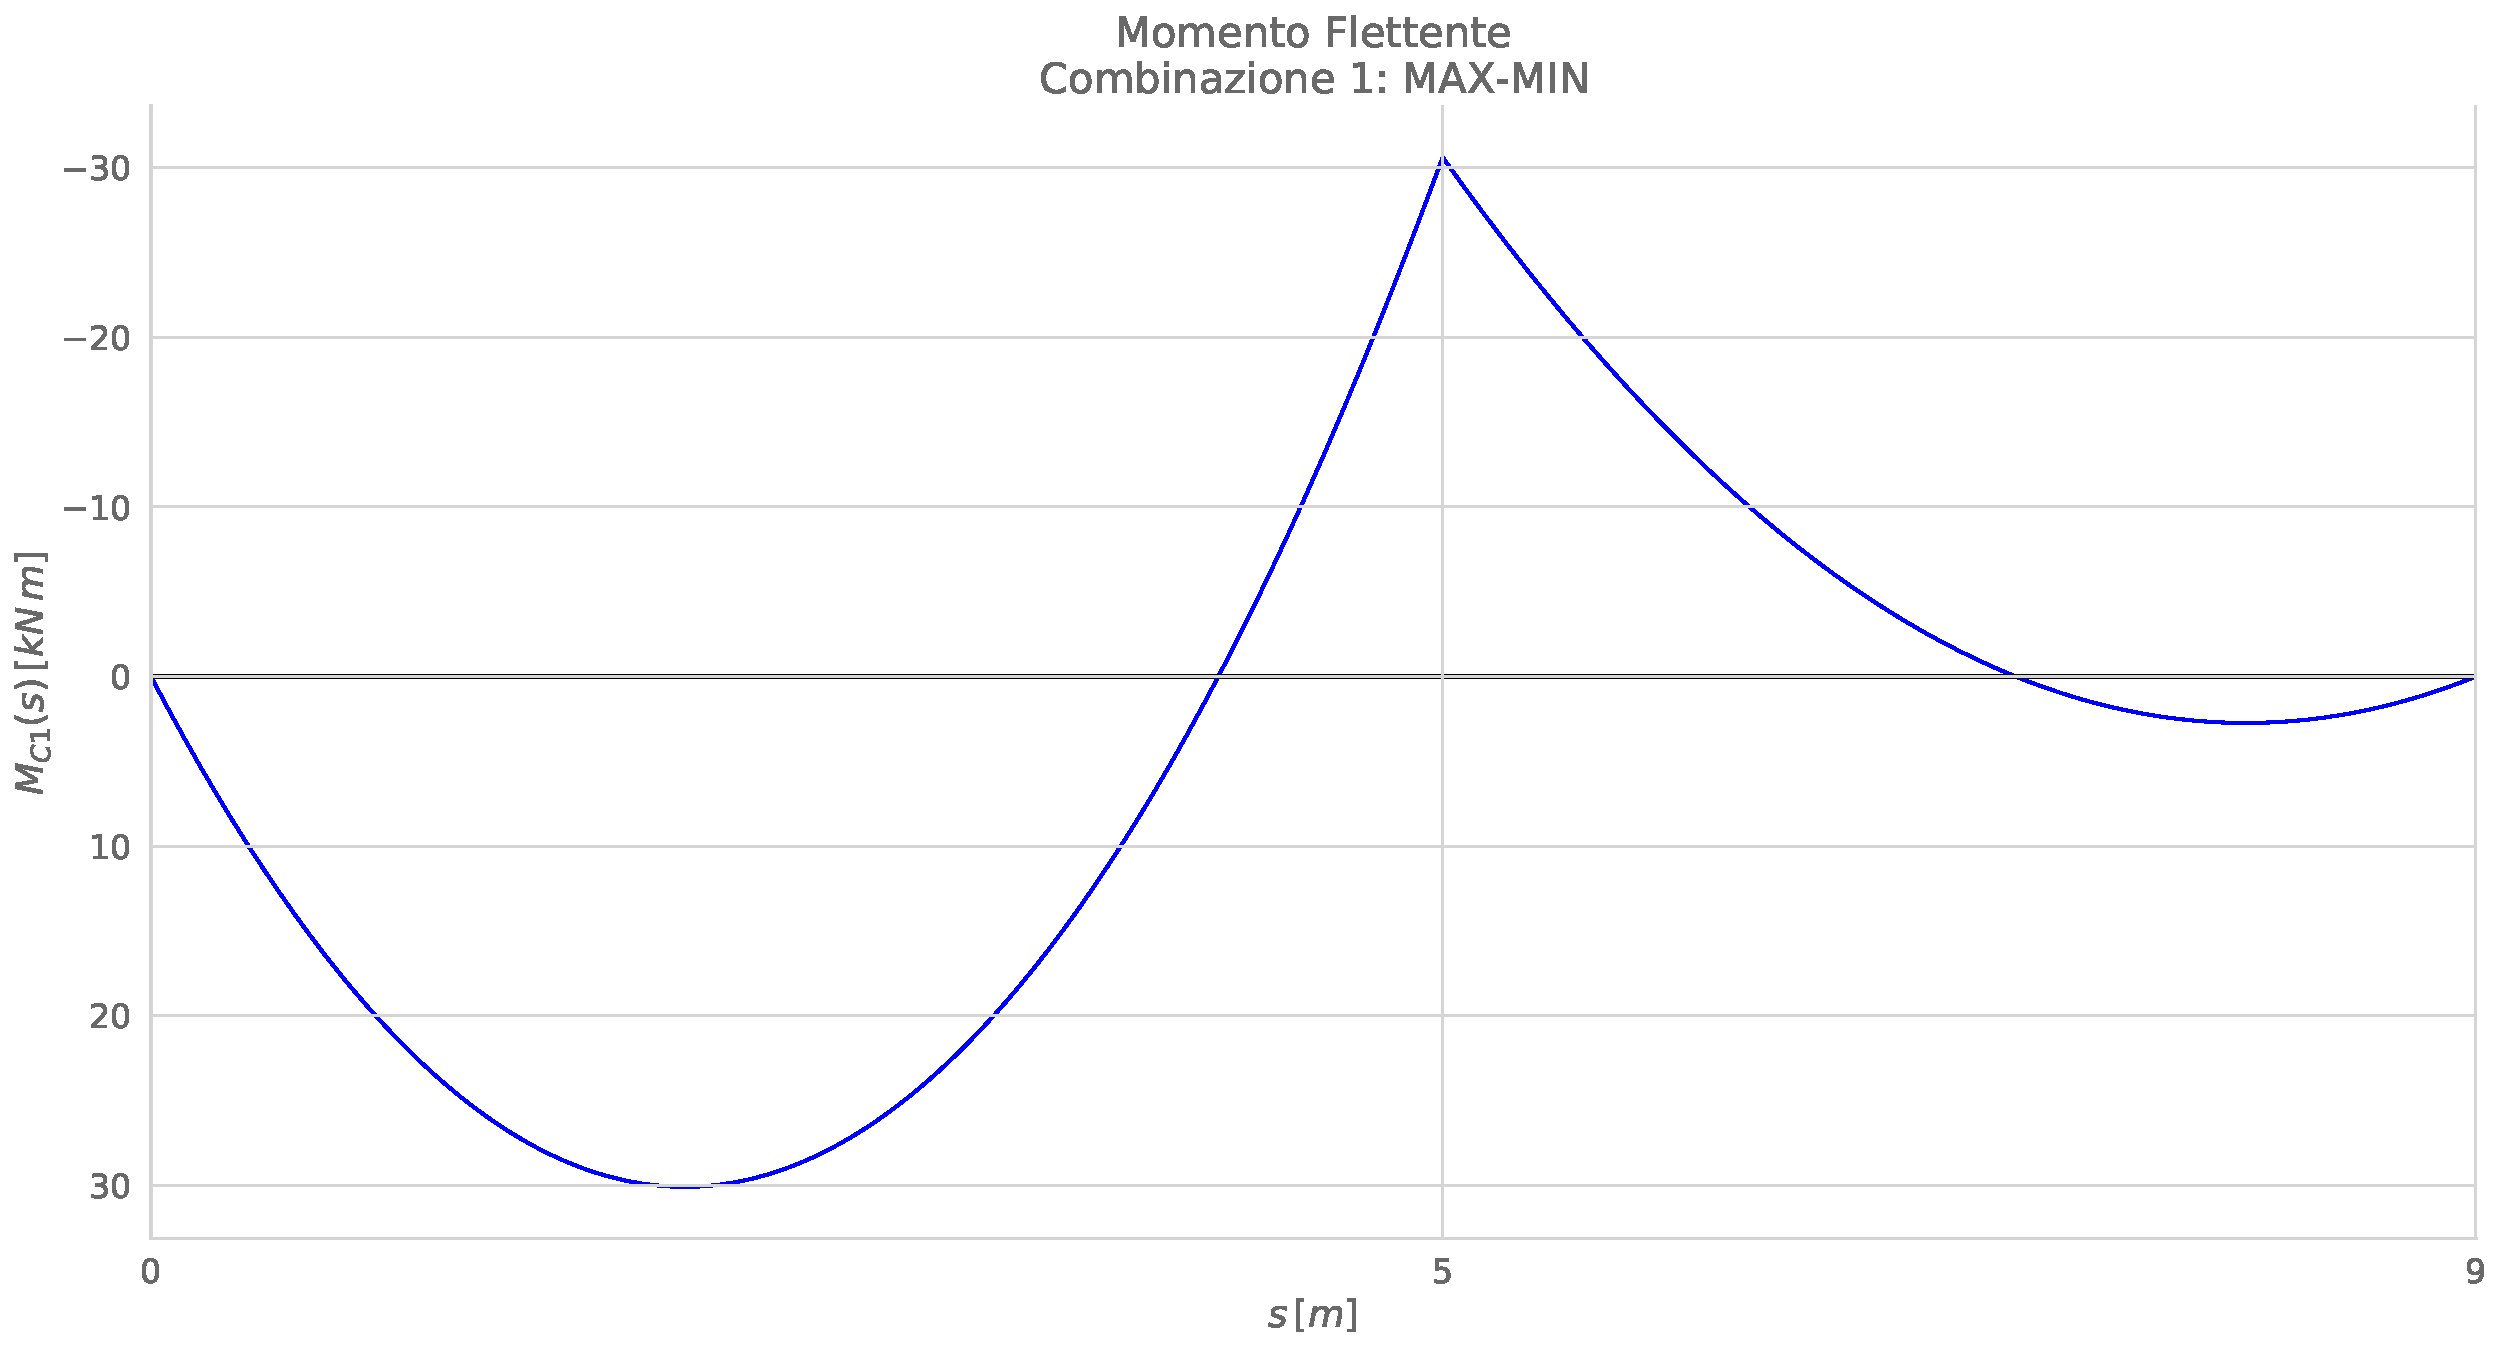
\includegraphics[width=\textwidth]{../../export/img/bendingMomentCombo_1}
 	\caption{Combinazione 1 che massimizza il momento flettente in campata $C1$}
 	\label{fig:bendingMomentCombo_1}
 \end{figure}

 Come si può capire, ogni combinazione origina un diagramma simile a quello riportato sopra. La figura~\ref{fig:bendingMomentComparison_slu} sovrappone i diagrammi dei momenti flettenti delle otto combinazioni, da cui deriverà il diagramma dell'inviluppo.
 
 \begin{figure}
 	\centering
 	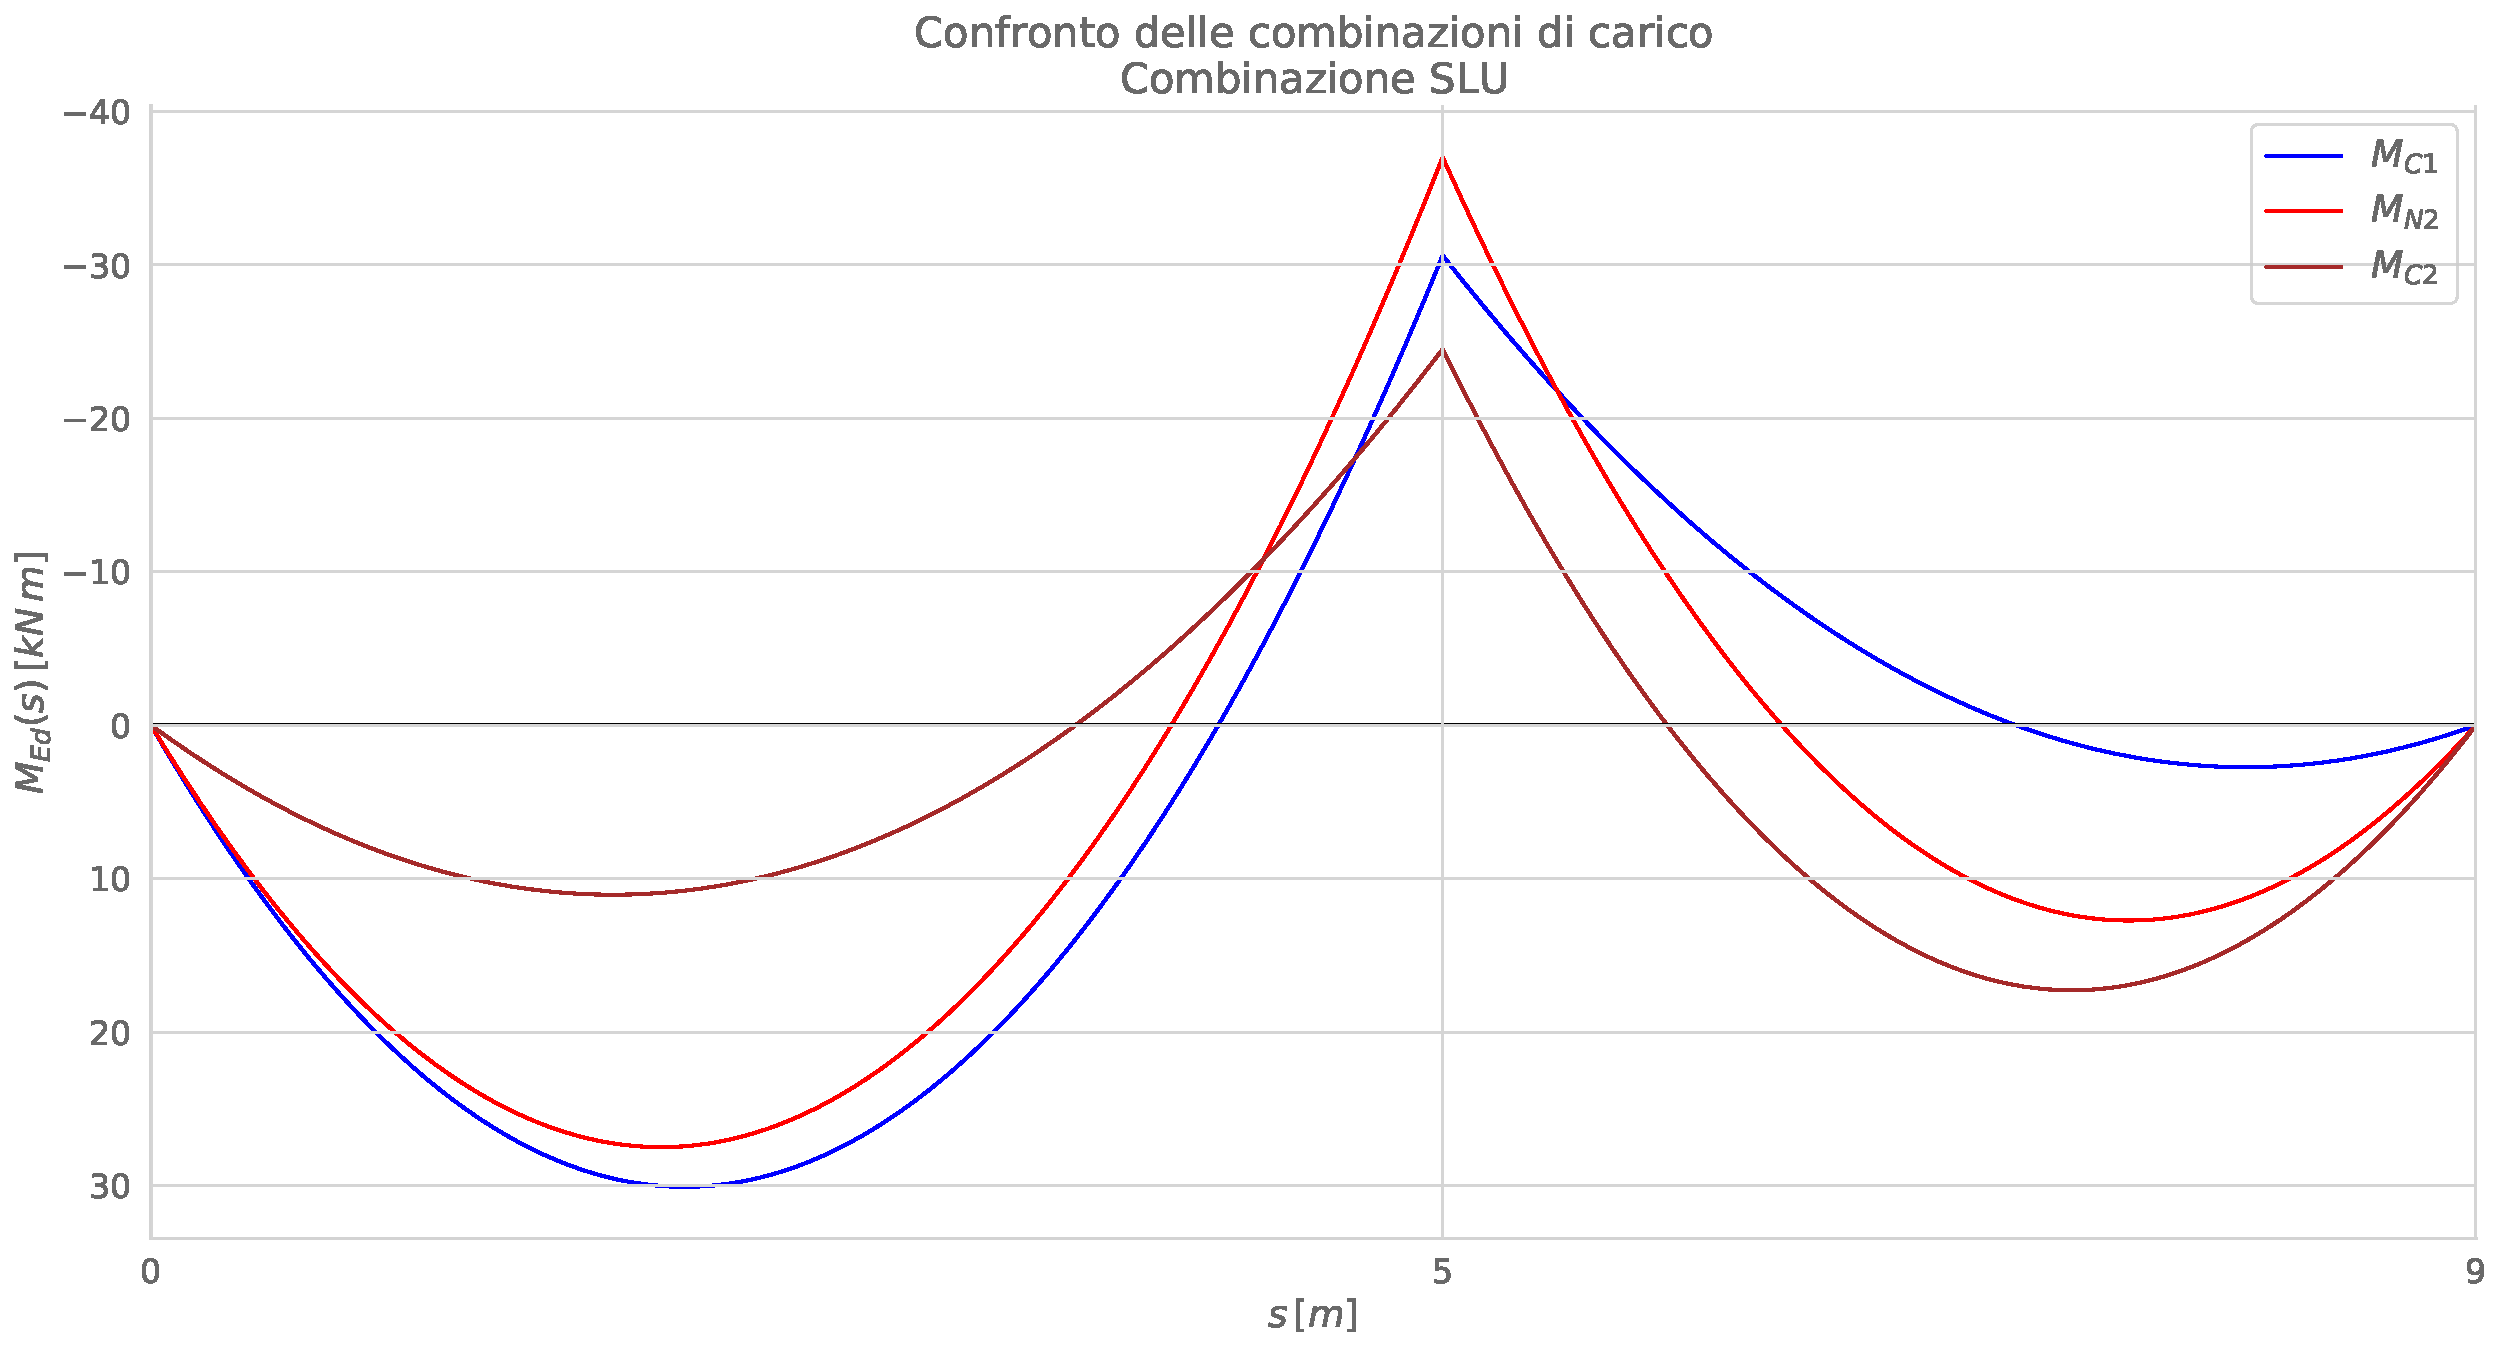
\includegraphics[width=\textwidth]{../../export/img/bendingMomentComparison_slu}
 	\caption{Confronto delle combinazioni}
 	\label{fig:bendingMomentComparison_slu}
 \end{figure}
 
 L'inviluppo dei momenti flettenti, è stato riprodotto attraverso il seguente stralcio di codice:
 
 \begin{lstlisting}[language=Python]
Mmax = np.zeros(1000)
Mmin = np.zeros(1000)

for i in range (0, 999):
    Mmax[i] = max(MC1[i], MN2[i], MC2[i], MN3[i], MC3[i], MN4[i], MN5[i], MN6[i])
    if Mmax[i] < 0:
        Mmax[i]=0
    Mmin[i] = min(MC1[i], MN2[i], MC2[i], MN3[i], MC3[i], MN4[i], MN5[i], MN6[i])
    if Mmin[i] > 0:
        Mmin[i]=0

#--------------------------------------

def bendingMomentPlot():
    plt.figure(figsize=(20,10))
    plt.fill(s, Mmax, linewidth='3', color='#0f0f0f80')
    plt.fill(s, Mmin, linewidth='3', color='#0f0f0f80')
    plt.xlim(s.min(), s.max())
    plt.gca().invert_yaxis()
    plt.grid()
    plt.xlabel(r'$s\,[m]$', fontsize='14')
    plt.ylabel(r'$M(s)\,[kN\,m]$', fontsize='14')
    plt.xticks([0, 3, 7.5, 11.5, 16.5, 22.65, 26.65,
    round(sC1max, 2), round(sC2max, 2), round(sC3max, 2), round(sC3max, 2), round(sC4max, 2), round(sC5max, 2), round(sC6max, 2)])
    plt.yticks(np.arange(-300, 250, step=50))
    plt.title('Inviluppo dei Momenti Flettenti\nCombinazione SLU', fontsize='22')
    plt.savefig('export/img/bendingMomentEnvelope_slu.jpg')
    return plt.show()

bendingMomentPlot()
 \end{lstlisting}
 che prende in input i valori dei momenti flettenti delle otto combinazioni e riporta in output i massimi positivi e negativi tra tulle le combinazioni.
 
 Ne deriva la figura~\ref{fig:bendingMomentEnvelope_slu} di pagina~\pageref{fig:bendingMomentEnvelope_slu}.
 
 \begin{figure}
 	\centering
 	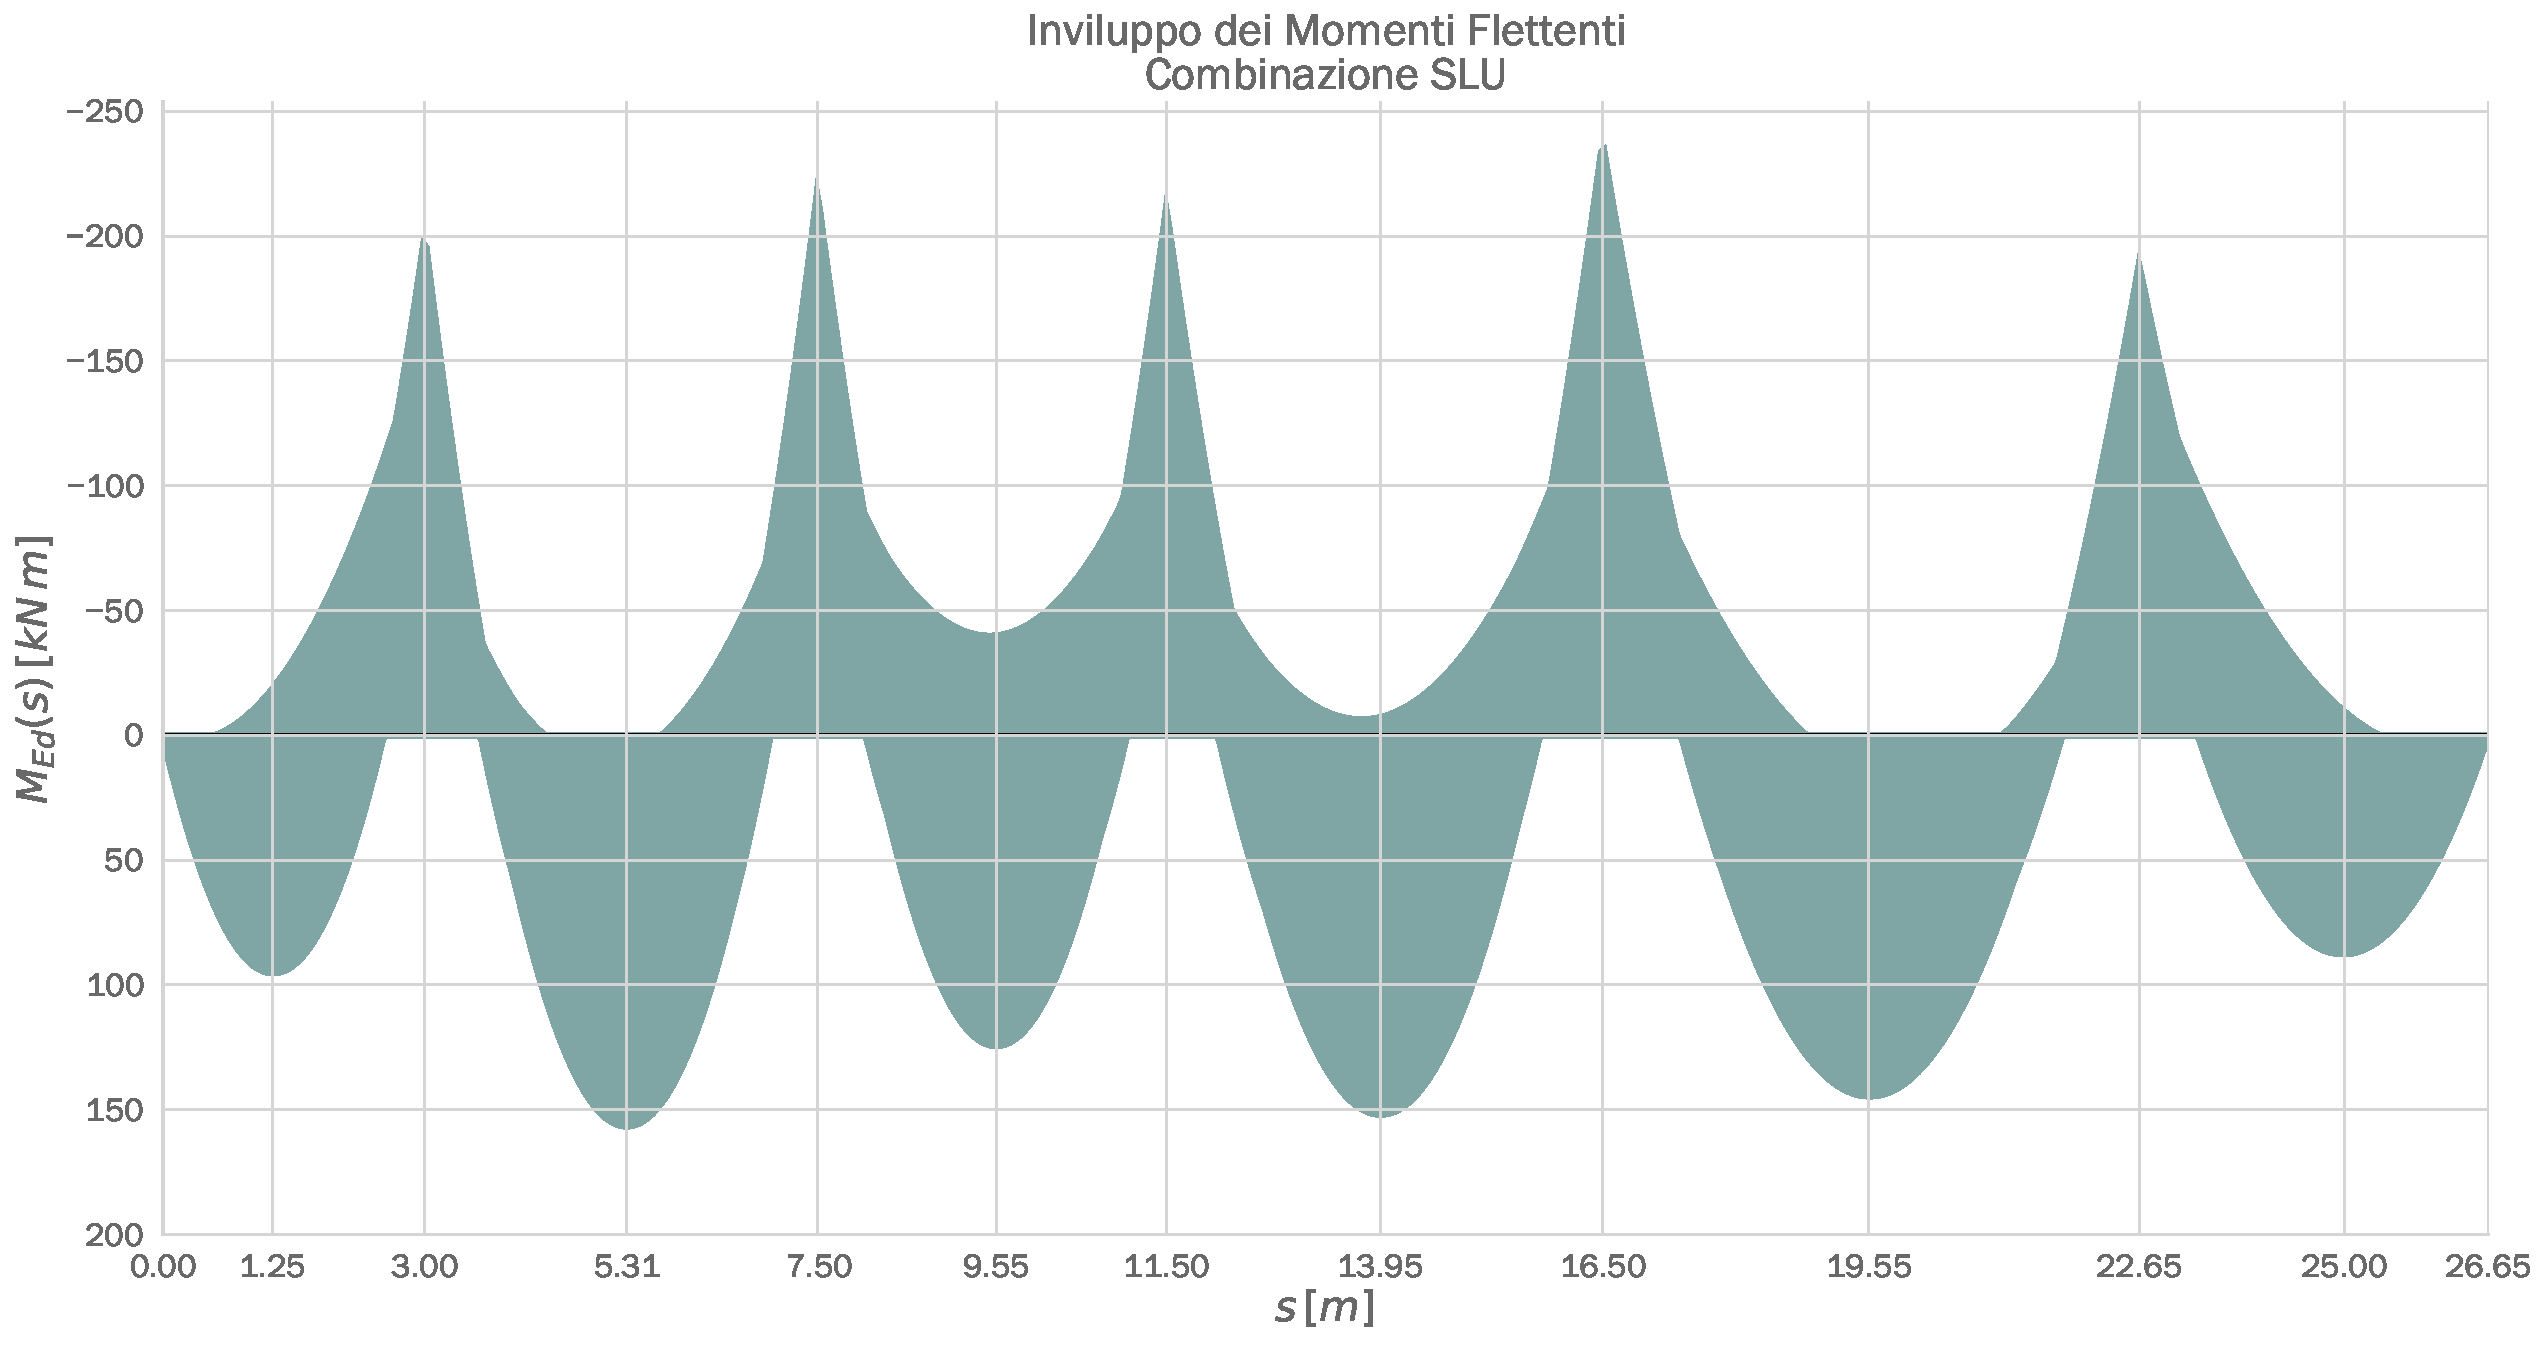
\includegraphics[width=\textwidth]{../../export/img/bendingMomentEnvelope_slu}
 	\caption{Diagramma dell'inviluppo dei momenti flettenti -- Combinazione SLU}
 	\label{fig:bendingMomentEnvelope_slu}
 \end{figure}

 Per comodità, in tabella~\ref{tab:max_min_bendingMomentEnvelope_slu} si riportano i valori massimi e minimi relativi dell'inviluppo e la coordinata $s$ corrispondente.
 
  \begin{table}
  	\centering
  	\caption{Valori massimi e minimi dell'inviluppo dei momenti}
  	\label{tab:max_min_bendingMomentEnvelope_slu}
  	\begin{tabular}{lcccr}
		\toprule
		& $M_{Ed}^+\,[kN\,m]$ & $s_{max}\,[m]$ & $M_{Ed}^-\,[kN\,m]$ & $s_{min}\,[m]$ \\
		Sezione &             &          &             &          \\
		\midrule
		C1      &     95.3533 &     1.25 &         NaN &      NaN \\
		N2      &         NaN &      NaN &     -196.35 &        3 \\
		C2      &     156.371 &     5.31 &           0 &      NaN \\
		N3      &         NaN &      NaN &    -217.324 &      7.5 \\
		C3      &     126.402 &     9.58 &    -38.9462 &      9.5 \\
		N4      &         NaN &      NaN &    -207.946 &     11.5 \\
		C4      &      149.47 &    13.93 &    -11.0069 &    13.61 \\
		N5      &         NaN &      NaN &    -251.747 &     16.5 \\
		C5      &     165.908 &    19.55 &           0 &      NaN \\
		N6      &         NaN &      NaN &    -215.246 &    22.65 \\
		C6      &     97.7052 &       25 &         NaN &      NaN \\
		\bottomrule
	\end{tabular}
  \end{table}

  \cleardoublepage
  Per l'azione interna di tipo tagliante, si procede analogamente al momento flettente, e si ottiene la figura~\ref{fig:shearEnvelope_slu} e la tabella~\ref{tab:shearEnvelope_slu}.
  
  \begin{figure}
 	\centering
 	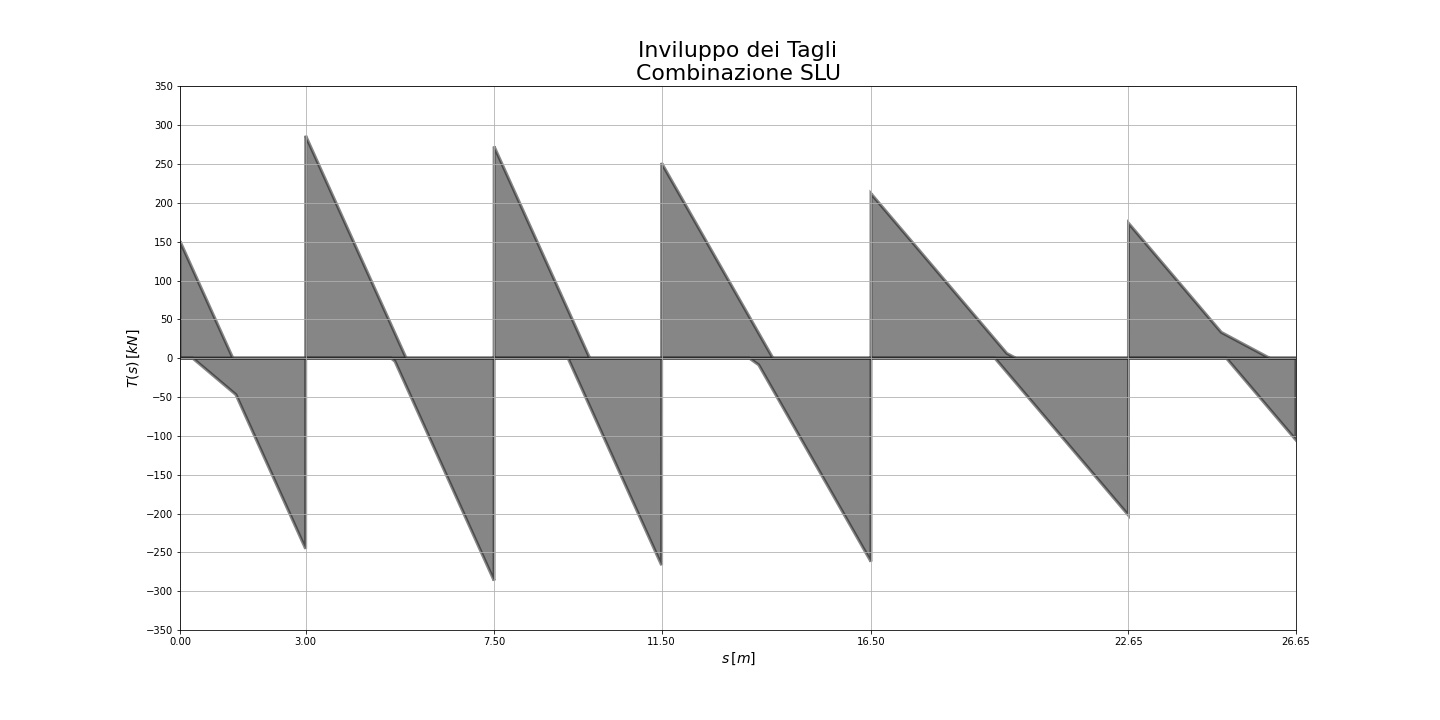
\includegraphics[width=\textwidth]{../../export/img/shearEnvelope_slu}
 	\caption{Diagramma dell'inviluppo dei tagli -- Combinazione SLU}
 	\label{fig:shearEnvelope_slu}
 \end{figure}
 
 \begin{table}
  	\centering
  	\caption{Valori massimi e minimi dell'inviluppo dei tagli}
  	\label{tab:shearEnvelope_slu}
  	\begin{tabular}{lcccr}
		\toprule
		& $T_{Ed}^+\,[kN]$ & $s_{max}\,[m]$ & $T_{Ed}^-\,[kN]$ & $s_{min}\,[m]$ \\
		Sezione &             &          &             &          \\
		\midrule
		N1      &   147.662 &        0 &         0 &        0 \\
		N2      &    284.68 &        3 &  -243.948 &        3 \\
		N3      &   271.689 &      7.5 &  -286.264 &      7.5 \\
		N4      &   247.323 &     11.5 &  -265.575 &     11.5 \\
		N5      &   237.551 &     16.5 &  -265.248 &     16.5 \\
		N6      &   196.751 &    22.65 &  -231.277 &    22.65 \\
		N7      &         0 &    26.65 &  -116.965 &    26.65 \\
		\bottomrule
	\end{tabular}
  \end{table}
  

  
